\documentclass[11pt,a4paper]{article}
\usepackage{amsmath}
\usepackage{amssymb}
\usepackage{xcolor}
\usepackage{tikz}
\usetikzlibrary{arrows,automata}

\begin{document}

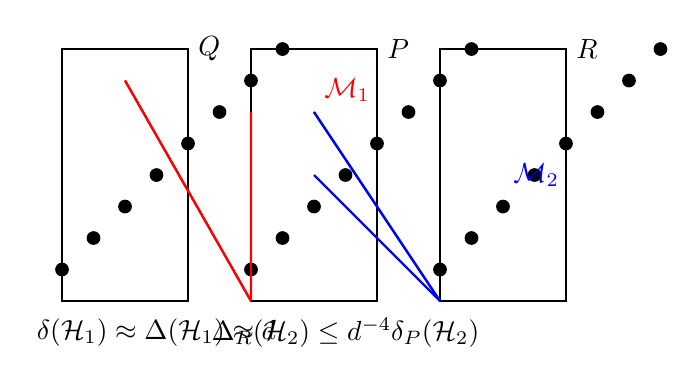
\begin{tikzpicture}[scale=0.8]
    % Define coordinates for nodes
    \coordinate (Q) at (0, 0);
    \coordinate (P) at (3, 0);
    \coordinate (R) at (6, 0);
    
    % Draw the hypergraph structure
    \draw[thick] (Q) rectangle ++(2, 4) node[right] {$Q$};
    \draw[thick] (P) rectangle ++(2, 4) node[right] {$P$};
    \draw[thick] (R) rectangle ++(2, 4) node[right] {$R$};
    
    % Draw vertices within each hyperedge
    \foreach \x in {0,...,7}{
        \filldraw[black, radius=0.1cm] (Q) ++(\x * 0.5, 0.5 + \x * 0.5) circle (0.1);
        \filldraw[black, radius=0.1cm] (P) ++(\x * 0.5, 0.5 + \x * 0.5) circle (0.1);
        \filldraw[black, radius=0.1cm] (R) ++(\x * 0.5, 0.5 + \x * 0.5) circle (0.1);
    }
    
    % Draw the matchings M_1 and M_2
    \draw[red, thick] (Q) ++(1, 3.5) -- (P) ++(1, 3);
    \draw[red, thick] (Q) ++(3, 3) -- (P) ++(1, 2);
    \draw[blue, thick] (P) ++(1, 3) -- (R) ++(1, 2);
    \draw[blue, thick] (P) ++(1, 2) -- (R) ++(1, 2);

    % Draw the matchings M_1 and M_2 with red and blue edges respectively
    \draw[red, thick] (Q) ++(1, 3.5) -- (P) ++(1, 3) node[above right]{$\mathcal{M}_1$};
    \draw[blue, thick] (P) ++(1, 3) -- (R) ++(1, 2) node[right]{$\mathcal{M}_2$};
    
    % Draw the labels
    \node at (1.5, -0.5) {$\delta(\mathcal{H}_1) \approx \Delta(\mathcal{H}_1) \approx d$};
    \node at (4.5, -0.5) {$\Delta_R(\mathcal{H}_2) \leq d^{-4}\delta_P(\mathcal{H}_2)$};

\end{tikzpicture}

Two matchings $\mathcal{M}_1 \subseteq \mathcal{H}_1$ and $\mathcal{M}_2 \subseteq \mathcal{H}_2$ in the hypergraph $\mathcal{H}$, whose union forms a $P$-perfect matching $\mathcal{M}$; here $p=2$, $q=4$, and $r=2$.